\section{Ligações elétricas residenciais}

\begin{frame}{Introdução}
	\begin{block}{Noções iniciais}
		\begin{itemize}
			\item As instalações elétricas tem um carácter muito \textbf{prático} nas nossas vidas: toda vez que \textbf{acendemos uma lâmpada}, ou \textbf{ligamos nosso celular ao carregador}, na tomada, estamos \textbf{utilizando} alguma \textbf{instalação elétrica}.
			\item Por mais abstrata que a disciplina pareça, a parte \textbf{prática} pode ser uma das mais importantes porque, se bem pensada, \textbf{facilita muito a vida de seus usuários}, que somos \textbf{nós}.
		\end{itemize}
	\end{block}

	\centering
	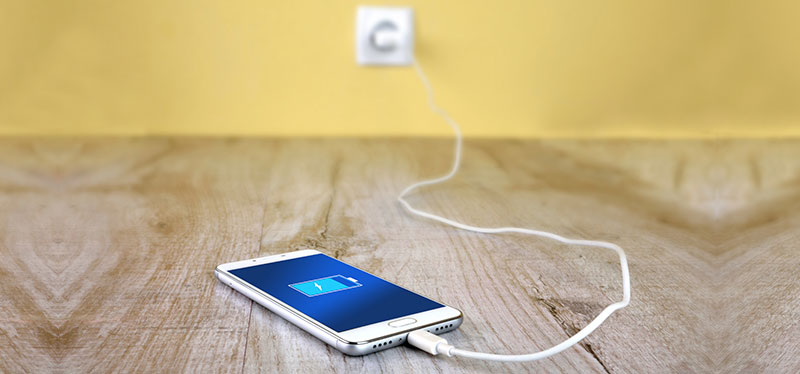
\includegraphics[width=0.65\linewidth]{Figuras/Ch08/fig12}
\end{frame}



\begin{frame}{Introdução}
	\begin{block}{Exemplo motivador}
		\begin{itemize}
			\item Imagine, por exemplo, que você chegou em casa e foi direto para o quarto, depois de um dia cheio.
			\item Acendeu a luz, mas esqueceu de apagá-la, \textbf{e agora?}
		\end{itemize}
	\end{block}

	\centering
	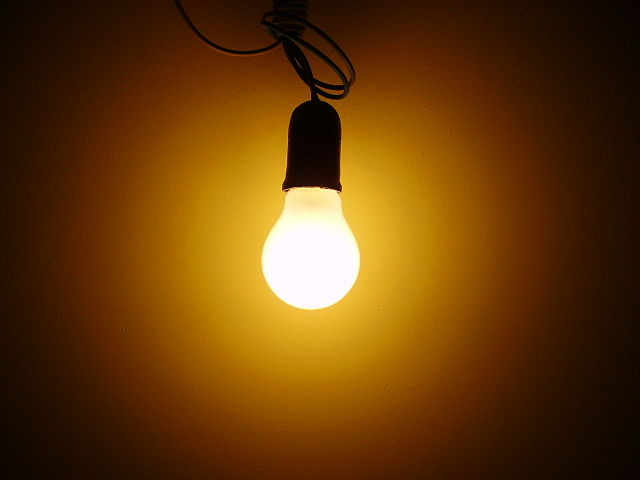
\includegraphics[width=0.6\linewidth]{Figuras/Ch08/fig13}
\end{frame}


\begin{frame}{Introdução}
	\begin{block}{Exemplo motivador}
		\begin{itemize}
			\item Nesse caso, uma das soluções possíveis seria o uso de dois interruptores em \textit{three-way}, que é um tipo de ligação que deixaria você ligar a lâmpada na porta do quarto e desligá-la em outro interruptor perto da cama.
			\item É esse o tipo de ligação que estudaremos nessa aula.
		\end{itemize}
	\end{block}

	%	\centering
	%	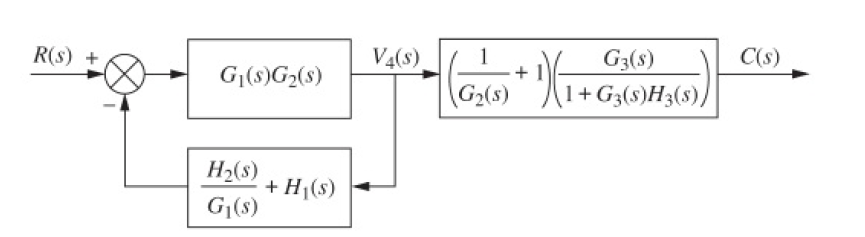
\includegraphics[width=0.6\linewidth]{Figuras/Ch08/fig29}
\end{frame}


\begin{frame}{Interruptores}
	\begin{block}{O que é?}
		\begin{itemize}
			\item O interruptor tem a função de \textbf{interromper a corrente elétrica do circuito}, de forma com que nas residências os interruptores são usados em \textbf{circuitos de iluminação}.
			\item Existem vários tipos de interruptores como por exemplo, interruptor simples, duplo, triplo, \textit{three way} (paralelo) e \textit{four way} (intermediário).
		\end{itemize}
	\end{block}

	\begin{minipage}{0.3\linewidth}
		\centering
		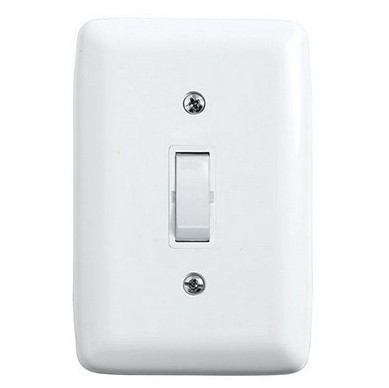
\includegraphics[height=0.5\textheight]{Figuras/Ch08/fig1}
	\end{minipage}\hfill
	\begin{minipage}{0.3\linewidth}
		\centering
		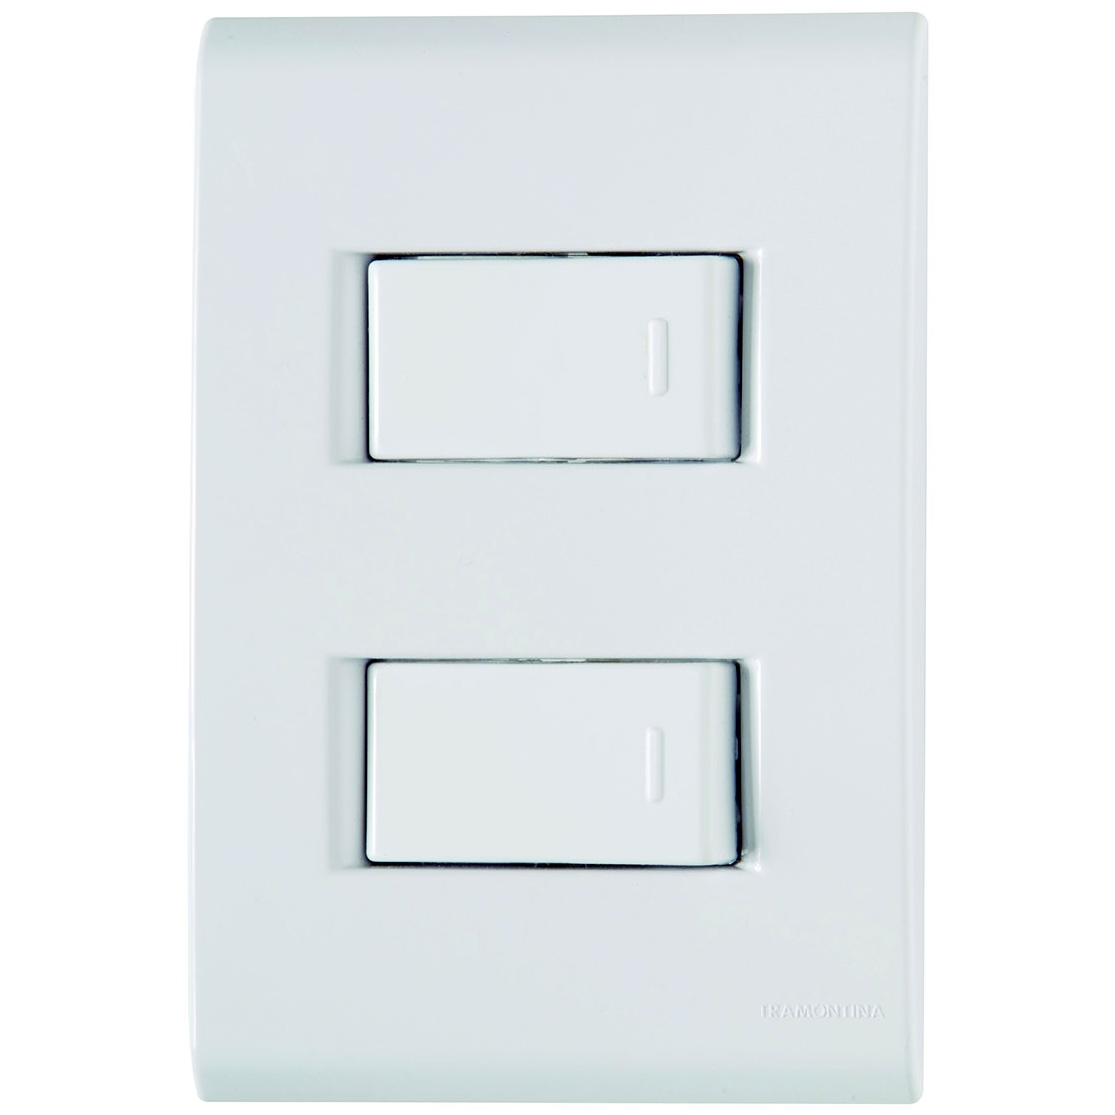
\includegraphics[height=0.45\textheight]{Figuras/Ch08/fig2}
	\end{minipage}\hfill
	\begin{minipage}{0.3\linewidth}
		\centering
		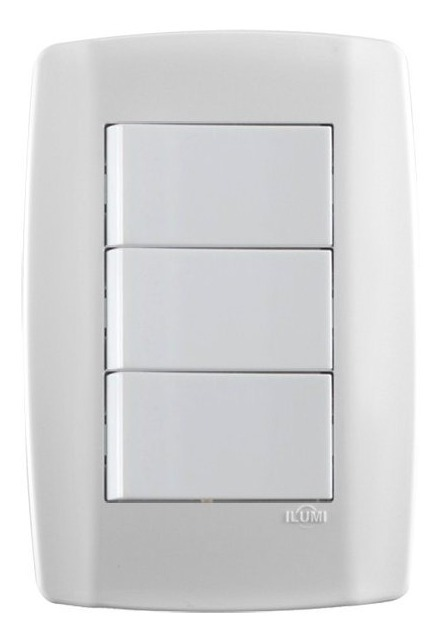
\includegraphics[height=0.5\textheight]{Figuras/Ch08/fig3}
	\end{minipage}

	%	\centering
	%	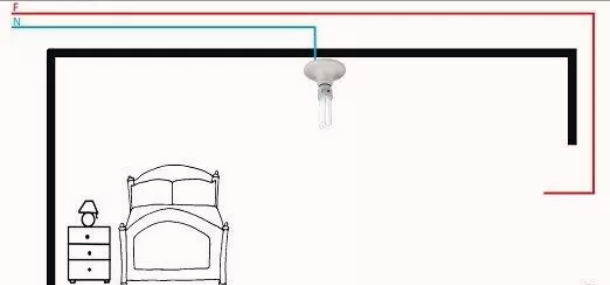
\includegraphics[width=0.6\linewidth]{Figuras/Ch08/fig18}
\end{frame}


\begin{frame}{Interruptores}
	\begin{block}{Interruptor simples}
		\begin{itemize}
			\item O \textbf{interruptor simples} têm a finalidade de acionar \textbf{uma lâmpada} ou \textbf{conjunto de lâmpadas} de \textbf{apenas um ponto}, possui \textbf{dois bornes}, sendo que em um borne é conectado o condutor elétrico \textbf{fase} e no outro borne o condutor de \textbf{retorno}, que vai para a lâmpada.
			\item É o interruptor \textbf{mais usado nas residências}.
		\end{itemize}
	\end{block}

	\begin{minipage}{0.48\linewidth}
		\centering
		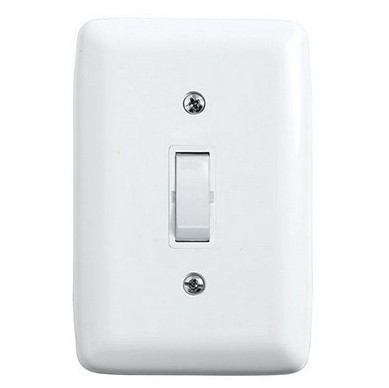
\includegraphics[height=0.5\textheight]{Figuras/Ch08/fig1}
	\end{minipage}\hfill
	\begin{minipage}{0.48\linewidth}
		\centering
		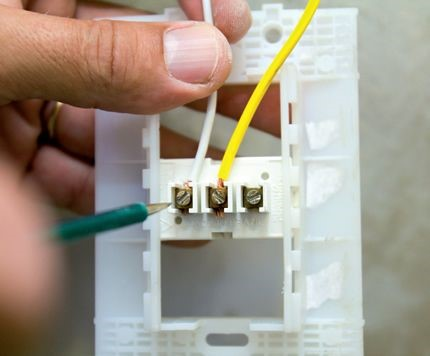
\includegraphics[height=0.5\textheight]{Figuras/Ch08/fig14}
	\end{minipage}
\end{frame}


\begin{frame}{Interruptores}
	\begin{block}{Interruptor duplo}
		\begin{itemize}
			\item O interruptor duplo possui duas seções e tem o \textbf{mesmo princípio} do interruptor simples, porém, podemos acionar \textbf{lâmpadas distintas}.
		\end{itemize}
	\end{block}

	\centering
	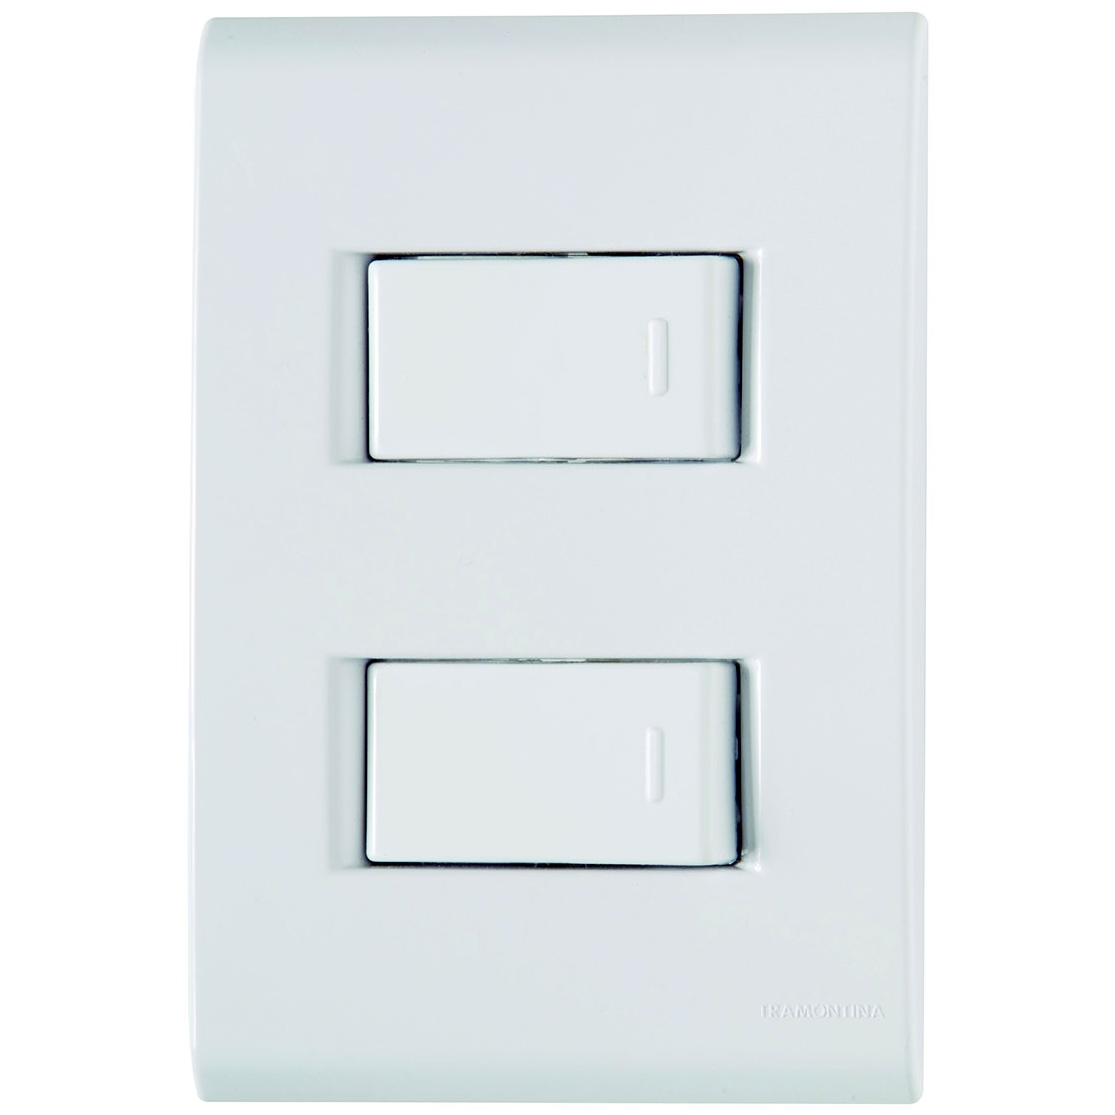
\includegraphics[height=0.7\textheight]{Figuras/Ch08/fig2}
\end{frame}


\begin{frame}{Interruptores}
	\begin{block}{Interruptor triplo}
		\begin{itemize}
			\item O interruptor triplo tem \textbf{o mesmo princípio} do interruptor duplo, mas \textbf{com uma seção a mais}.
			\item Muito usado em \textbf{salas muito amplas} e \textbf{cômodos conjugados}.
			\item É muito comum o uso do interruptor triplo em \textbf{galpões}, pois pode acionar três grupos de lâmpadas diferentes como, por exemplo, acionar a \textbf{parte da frente}, do \textbf{meio} ou \textbf{fundo do galpão} de \textbf{forma independente}.
		\end{itemize}
	\end{block}

	\centering
	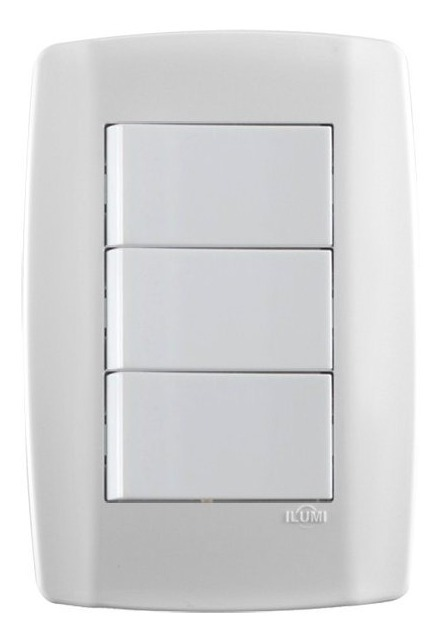
\includegraphics[height=0.4\textheight]{Figuras/Ch08/fig3}
\end{frame}


\begin{frame}{Interruptores - Arranjos}
	\begin{block}{\textit{Three Way} (paralelo)}
		\begin{itemize}
			\item O interruptor \textit{three way} mais conhecido como \textbf{interruptor paralelo}, é usado para acionar uma lâmpada ou um grupo de lâmpadas de \textbf{dois pontos diferentes}.
			\item Por estarem localizados em dois pontos diferentes, os interruptores \textit{three way} oferecem um maior \textbf{conforto} e \textbf{praticidade}.
		\end{itemize}
	\end{block}

	\centering
	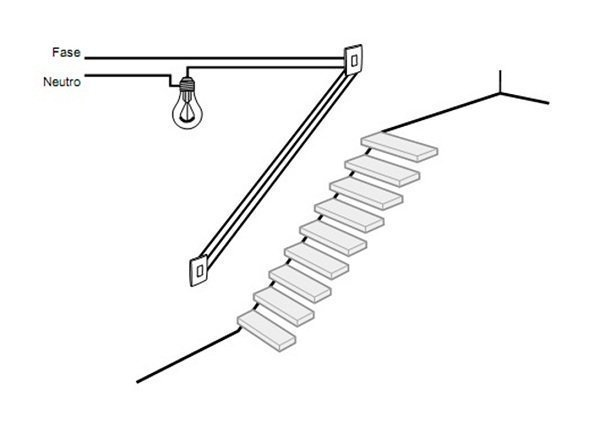
\includegraphics[width=0.55\linewidth]{Figuras/Ch08/fig4}
\end{frame}


\begin{frame}{Interruptores - Arranjos}
	\begin{block}{\textit{Three Way} (paralelo)}
		\begin{itemize}
			\item A diferença entre o interruptor \textit{three way} para o interruptor simples é a existência de um \textbf{terceiro borne}, que faz a comunicação entre os \textbf{dois interruptores \textit{three way}} ou entre \textbf{o interruptor \textit{three way} e o interruptor \textit{four way}}.
		\end{itemize}
	\end{block}

	\centering
	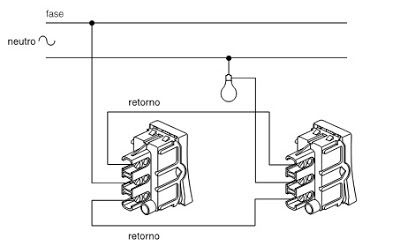
\includegraphics[width=0.6\linewidth]{Figuras/Ch08/fig5}
\end{frame}


\begin{frame}{Interruptores - Arranjos}
	\begin{block}{\textit{Four Way} (intermediário)}
		\begin{itemize}
			\item
			      O interruptor \textit{four way}, também conhecido como \textbf{interruptor intermediário}, deve ser ligado \textbf{entre dois interruptores \textit{three way}} para funcionar corretamente e assim \textbf{ampliando os pontos de acionamento das lâmpadas}, possibilitando ter \textbf{três ou mais pontos de acionamento} de lâmpada ou grupo de lâmpada sendo acionados.
		\end{itemize}
	\end{block}

	\vspace{0.5cm}

	\centering
	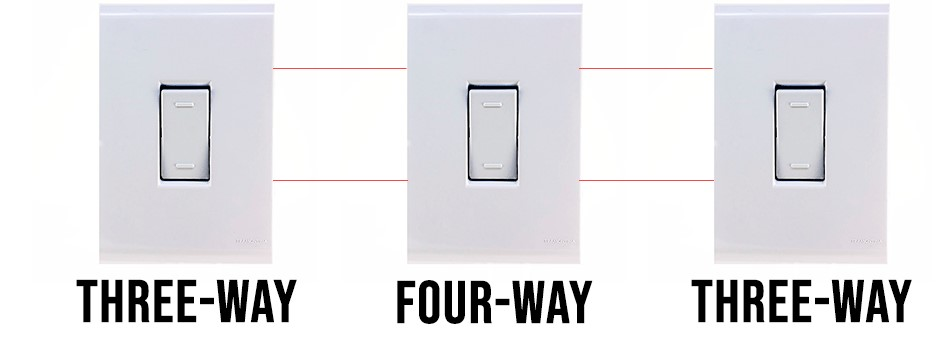
\includegraphics[width=0.6\linewidth]{Figuras/Ch08/fig15}
\end{frame}


\begin{frame}{Interruptores - Arranjos}
	\begin{block}{Diferenças}
		\begin{itemize}
			\item As diferenças entre os interruptores são:
			      \begin{itemize}
				      \item\normalsize quantidade de \textbf{pontos de ligação};
				      \item\normalsize quantidade de \textbf{bornes}, e;
				      \item\normalsize quantidade de \textbf{seções}.
			      \end{itemize}
			\item O interruptor \textbf{simples}, \textbf{duplo} e \textbf{triplo} possibilitam acender ou apagar uma lâmpada \textbf{somente de um ponto}.
			\item Porém, os interruptores duplo e triplo possuem \textbf{seções a mais} do que o interruptor simples, assim acionando \textbf{diferentes conjuntos de lâmpadas}.
			\item Já com o interruptor \textit{three way}, pode ser acionar a lâmpada de \textbf{dois pontos diferentes}, muito usado em escadas e corredores.
			\item \textit{Three way} X interruptor triplo: não faz sentido falar de \textbf{um \textit{three way}}, pois sempre vêm \textbf{aos pares}.
		\end{itemize}
	\end{block}

	%	\centering
	%	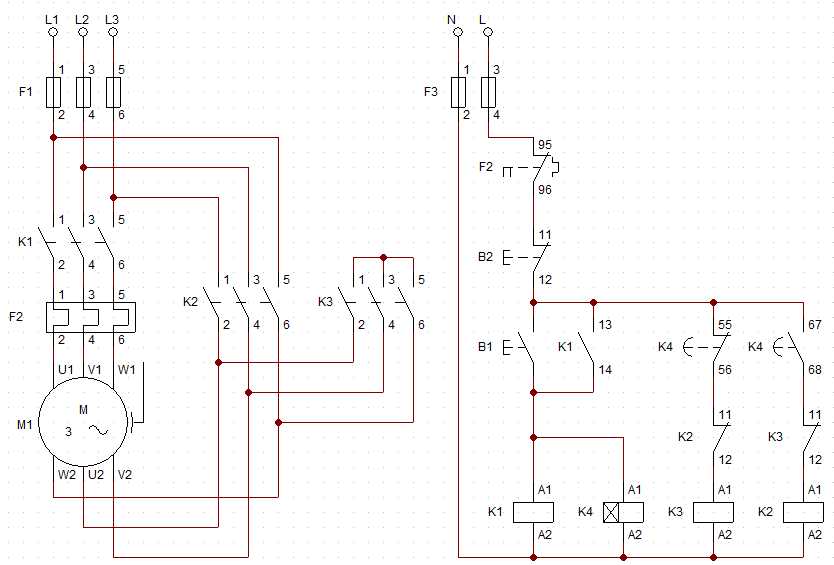
\includegraphics[width=0.6\linewidth]{Figuras/Ch08/fig22.jpg}
\end{frame}


\begin{frame}{Interruptores - Exemplo de ligação \#01}
	\begin{block}{\textit{Three way}}
		\begin{itemize}
			\item No quarto de uma residência, que já tinha um circuito de interruptor simples para o acionamento da lâmpada, o proprietário resolve instalar um \textit{three way}.
		\end{itemize}
	\end{block}

	\medskip

	\centering
	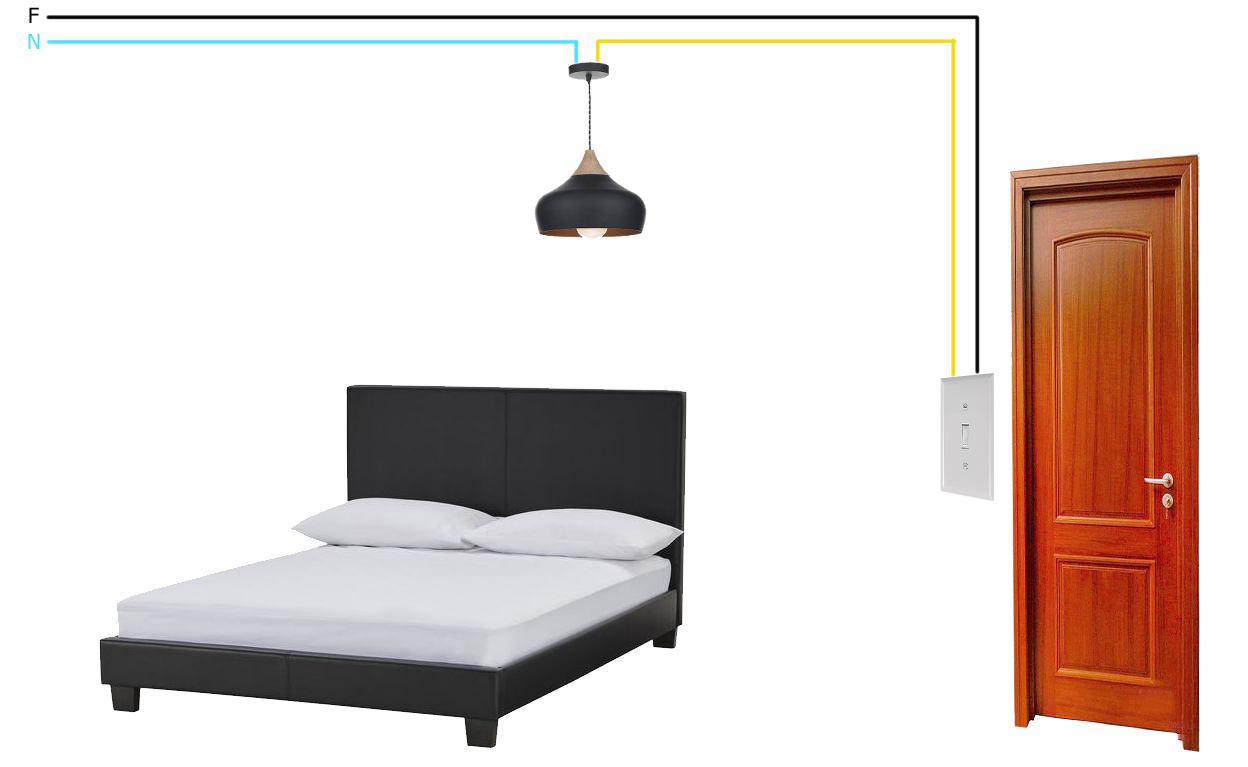
\includegraphics[width=0.7\linewidth]{Figuras/Ch08/fig16.1}
\end{frame}


\begin{frame}{Interruptores - Exemplo de ligação \#01}
	\begin{block}{\textit{Three way}}
		\begin{itemize}
			\item Na propriedade exemplificada a instalação possui tensão de \SI{127}{\volt} (fase e neutro).
			\item Devemos \textbf{sempre} conferir se é preciso passar novos eletrodutos.
			\item De qualquer forma, devemos adquirir \textbf{condutores} e \textbf{interruptores \textit{three way}}.
		\end{itemize}
	\end{block}

	\bigskip

	\centering
	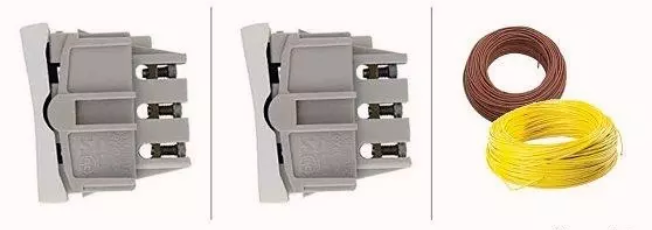
\includegraphics[width=0.7\linewidth]{Figuras/Ch08/fig17}
\end{frame}


\begin{frame}{Interruptores - Exemplo de ligação \#01}
	\begin{block}{\textit{Three way}}
		\begin{itemize}
			\item Após a compra dos materiais elétricos, por segurança, \textbf{desligamos o disjuntor} responsável pelo \textbf{circuito de iluminação}.
			\item Caso não exista separação de circuitos na propriedade, devemos \textbf{desligar o disjuntor geral}.
			\item Agora, retiramos o interruptor simples e o retorno da lâmpada do circuito com interruptor simples.
		\end{itemize}
	\end{block}

	\centering
	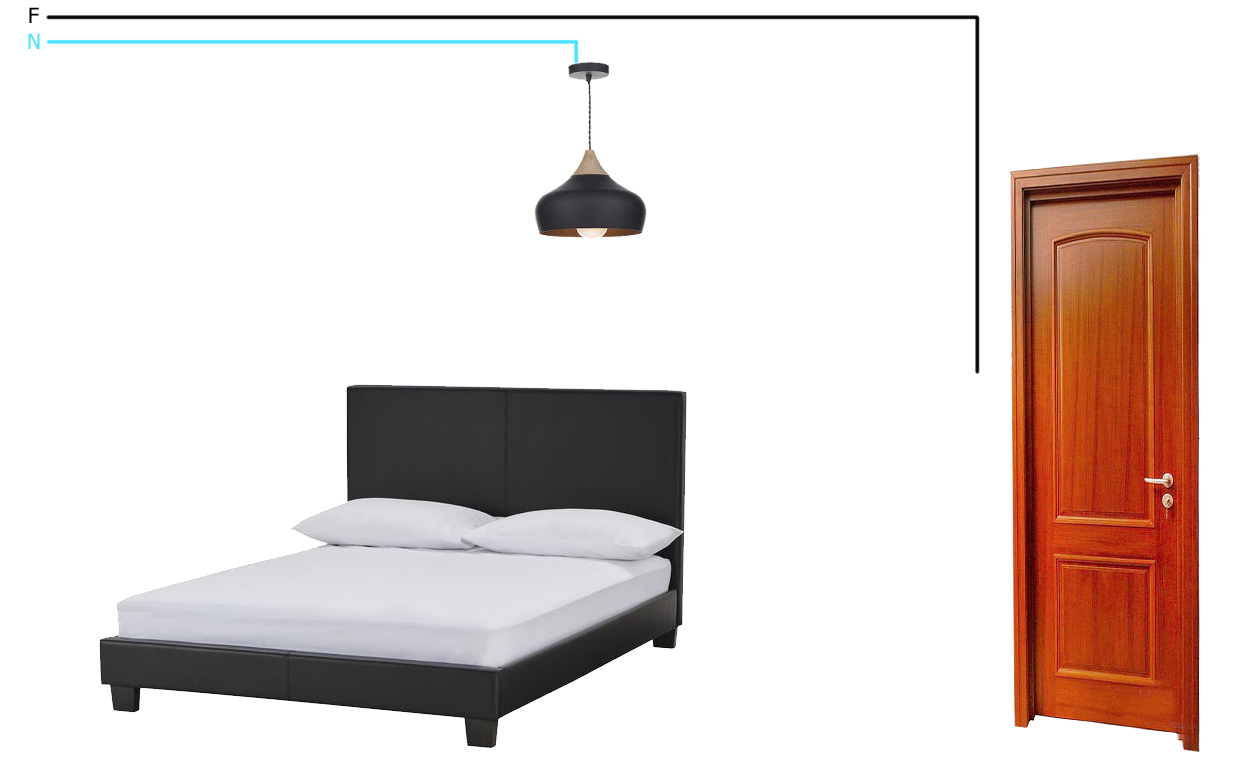
\includegraphics[width=0.5\linewidth]{Figuras/Ch08/fig18.1}
\end{frame}


\begin{frame}{Interruptores - Exemplo de ligação \#01}
	\begin{block}{\textit{Three way}}
		\begin{itemize}
			\item É preciso instalar o interruptor \textit{three way} no lugar do interruptor simples.
			\item Para isso, conectamos o condutor \textbf{fase} (vermelho), no borne \textbf{central} do interruptor \textit{three way} (A).
		\end{itemize}
	\end{block}

	\bigskip

	\centering
	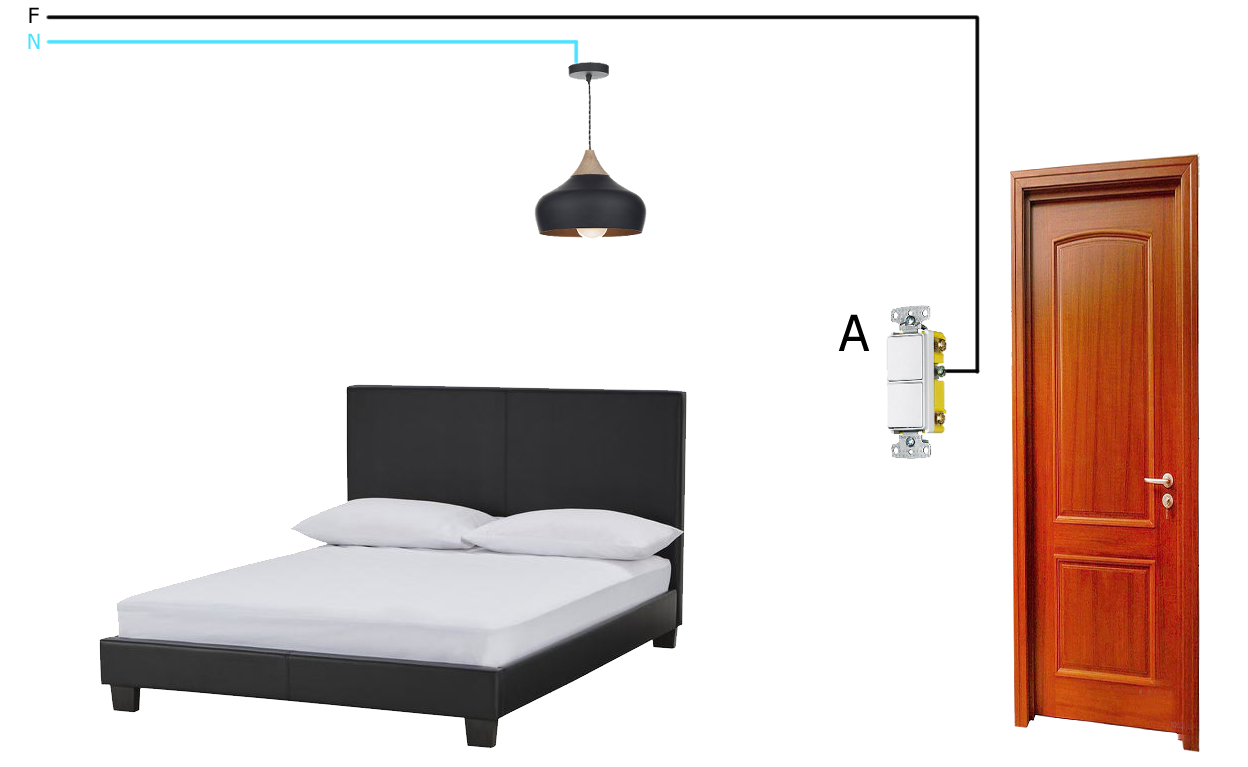
\includegraphics[width=0.6\linewidth]{Figuras/Ch08/fig19.1}
\end{frame}


\begin{frame}{Interruptores - Exemplo de ligação \#01}
	\begin{block}{\textit{Three way}}
		\begin{itemize}
			\item O próximo passo é escolher o melhor lugar para instalar o segundo interruptor \textit{three way} (B): no exemplo foi definido o ponto ao lado da cama.
		\end{itemize}
	\end{block}

	\bigskip

	\centering
	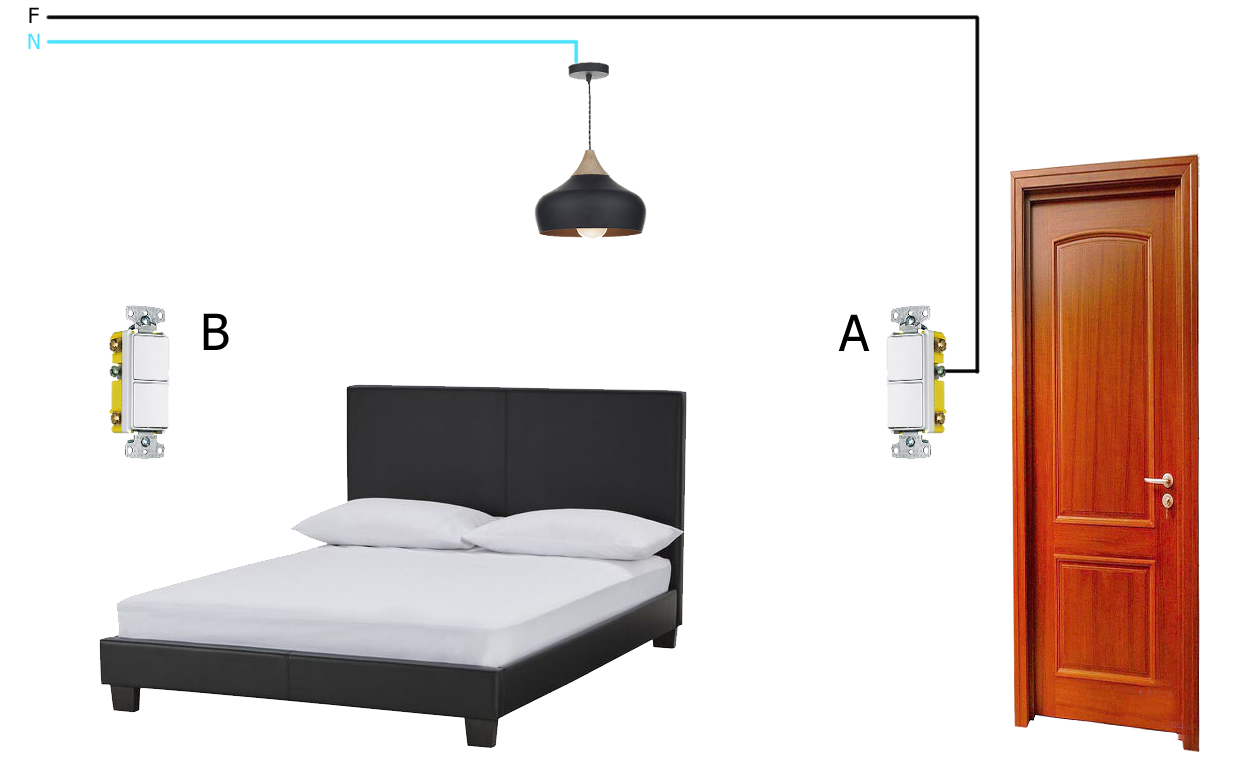
\includegraphics[width=0.7\linewidth]{Figuras/Ch08/fig20.1}
\end{frame}


\begin{frame}{Interruptores - Exemplo de ligação \#01}
	\begin{block}{\textit{Three way}}
		\begin{itemize}
			\item Em seguida devemos conectar o primeiro condutor elétrico (marrom 1), no borne \textbf{superior} do interruptor \textit{three way} (A), levando o condutor até o segundo interruptor \textit{three way} (B) e conectando o condutor no borne \textbf{superior} do interruptor \textit{three way} (B).
		\end{itemize}
	\end{block}

	\medskip

	\centering
	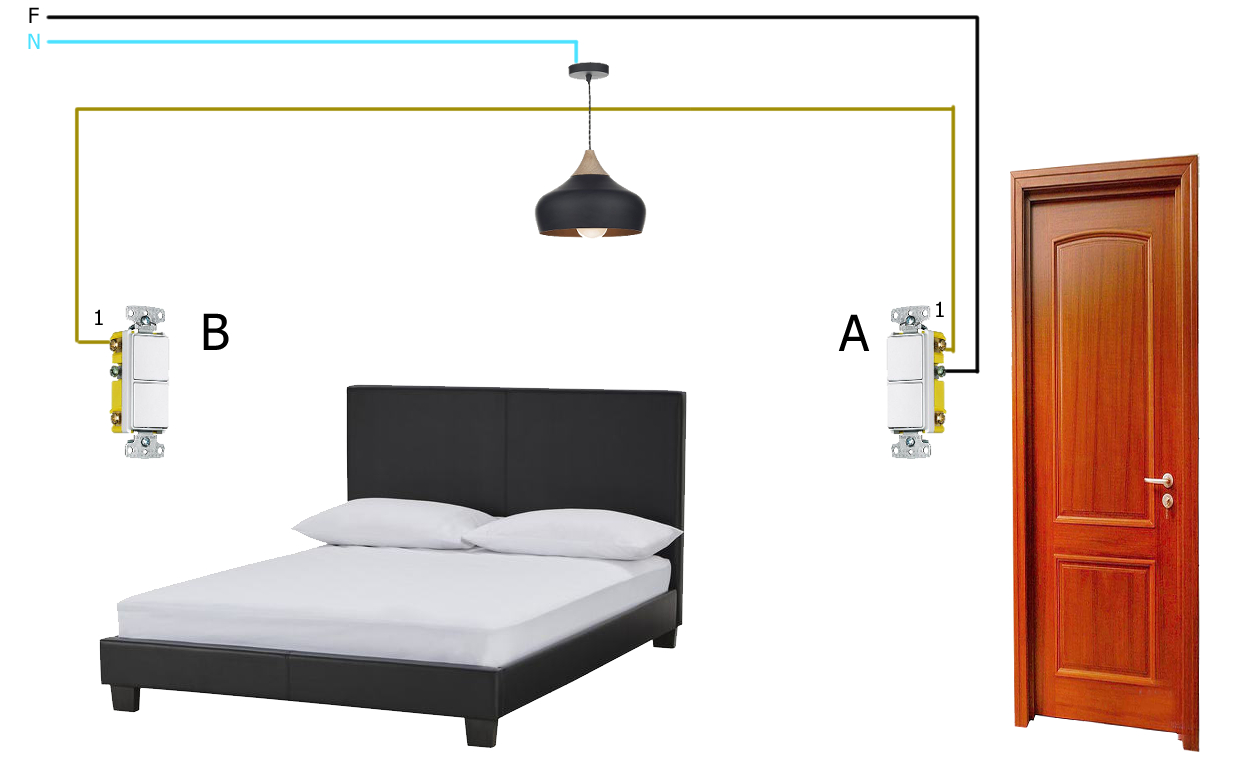
\includegraphics[width=0.65\linewidth]{Figuras/Ch08/fig20.2}
\end{frame}


\begin{frame}{Interruptores - Exemplo de ligação \#01}
	\begin{block}{\textit{Three way}}
		\begin{itemize}
			\item Em seguida é preciso conectar um segundo condutor elétrico (marrom 2), no borne \textbf{inferior} do interruptor (A), levando o segundo condutor elétrico até o interruptor (B), e conectando o condutor no borne \textbf{inferior} do interruptor \textit{three way} (B).
		\end{itemize}
	\end{block}

	\medskip

	\centering
	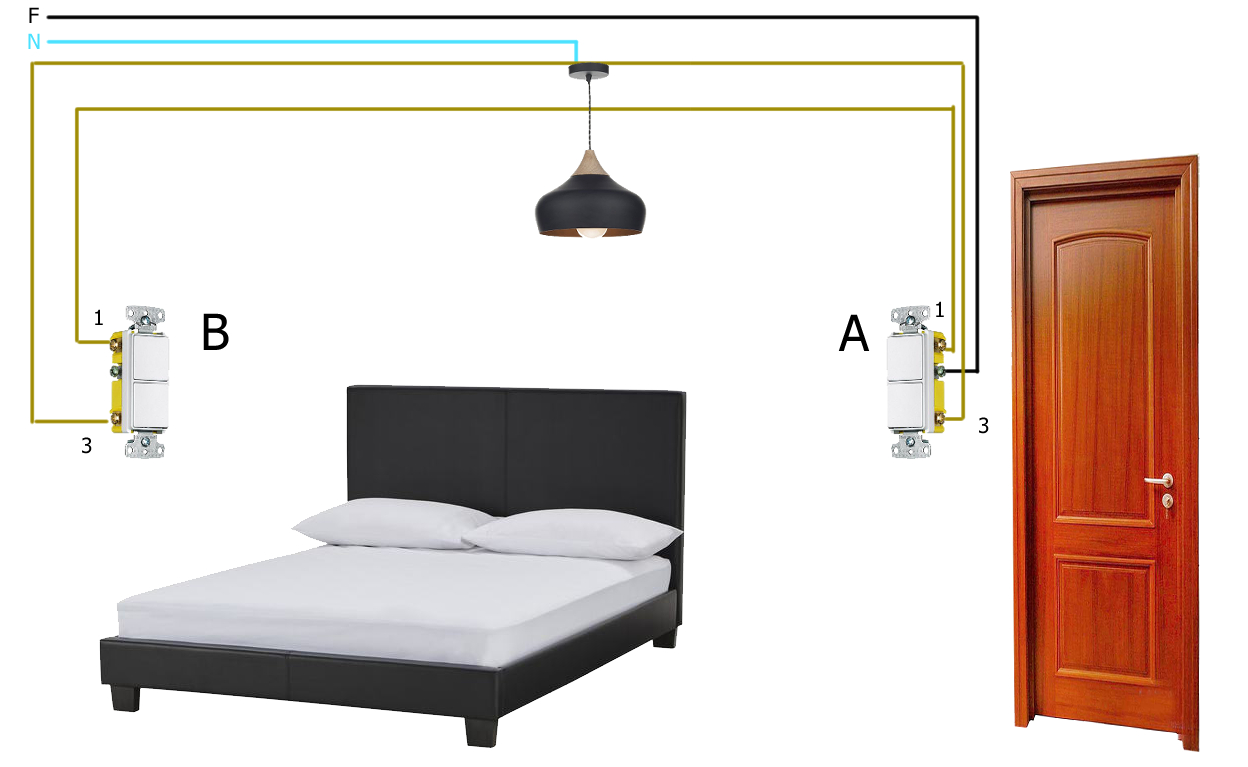
\includegraphics[width=0.65\linewidth]{Figuras/Ch08/fig20.3}
\end{frame}


\begin{frame}{Interruptores - Exemplo de ligação \#01}
	\begin{block}{\textit{Three way}}
		\begin{itemize}
			\item Para finalizar a ligação do circuito dos interruptores \textit{three way} é preciso conectar um condutor elétrico (retorno amarelo) no borne \textbf{central} do interruptor \textit{three way} e conectá-lo no borne \textbf{central} do \textbf{receptáculo} (soquete ou boquilha).
			\item Após ter concluído a instalação podemos ligar o disjuntor novamente, e agora é possível acionar a lâmpada de dois pontos distintos.
		\end{itemize}
	\end{block}

	\centering
	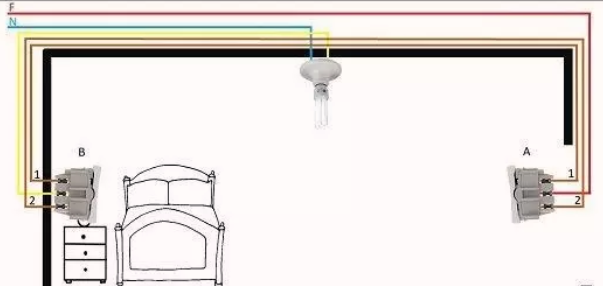
\includegraphics[width=0.6\linewidth]{Figuras/Ch08/fig21}
\end{frame}


\begin{frame}{Interruptores - Exemplo de ligação \#02}
	\begin{block}{\textit{Four way}}
		\begin{itemize}
			\item Para fazer a instalação do interruptor \textit{four way} é preciso entender a ligação do interruptor \textit{three way}.
			\item A instalação simples de um interruptor intermediário é feita usando apenas \textbf{dois interruptores paralelos}.
		\end{itemize}
	\end{block}

	\bigskip

	\centering
	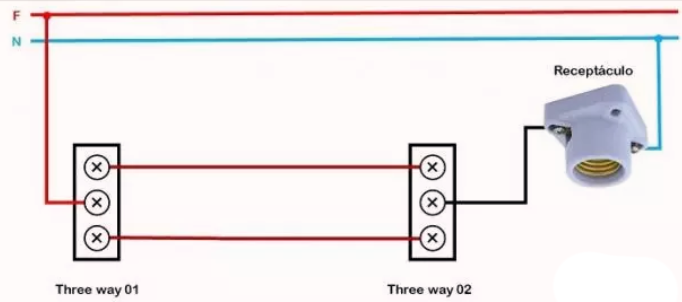
\includegraphics[width=0.8\linewidth]{Figuras/Ch08/fig22}
\end{frame}


\begin{frame}{Interruptores - Exemplo de ligação \#02}
	\begin{block}{\textit{Four way}}
		\begin{itemize}
			\item Devemos ligar o borne \textbf{central} do interruptor 1 ao condutor \textbf{fase}, em seguida ligamos um cabo do borne \textbf{central} do interruptor 2 ao borne \textbf{central} do \textbf{receptáculo} e, por último, ligamos ao borne \textbf{lateral} do \textbf{receptáculo} o condutor \textbf{neutro}.
		\end{itemize}
	\end{block}

	\bigskip

	\centering
	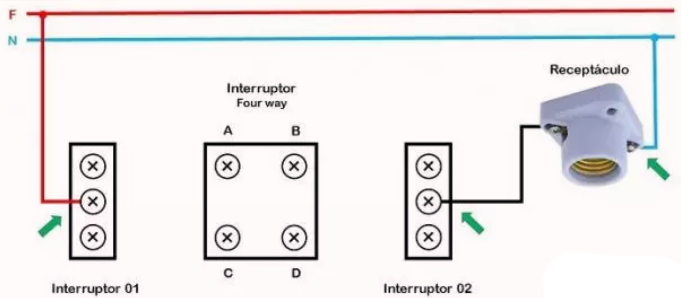
\includegraphics[width=0.8\linewidth]{Figuras/Ch08/fig23}
\end{frame}


\begin{frame}{Interruptores - Exemplo de ligação \#02}
	\begin{block}{\textit{Four way}}
		\begin{itemize}
			\item Devemos ligar um cabo do borne \textbf{superior} do interruptor 1 ao borne “A” do \textbf{interruptor intermediário}, em seguida ligamos um cabo do borne \textbf{inferior} do interruptor 1 ao borne “C” do \textbf{interruptor intermediário}.
		\end{itemize}
	\end{block}

	\bigskip

	\centering
	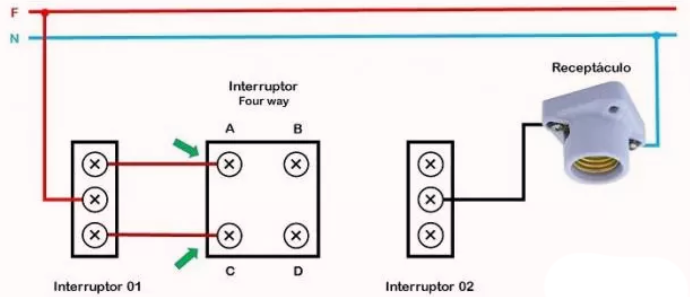
\includegraphics[width=0.8\linewidth]{Figuras/Ch08/fig24}
\end{frame}


\begin{frame}{Interruptores - Exemplo de ligação \#02}
	\begin{block}{\textit{Four way}}
		\begin{itemize}
			\item Por último ligamos um cabo do borne \textbf{superior} do interruptor 2 ao borne “B” do \textbf{interruptor intermediário}, em seguida ligamos um cabo do borne \textbf{inferior} do interruptor 2 ao borne “D” do \textbf{interruptor intermediário}.
		\end{itemize}
	\end{block}

	\bigskip

	\centering
	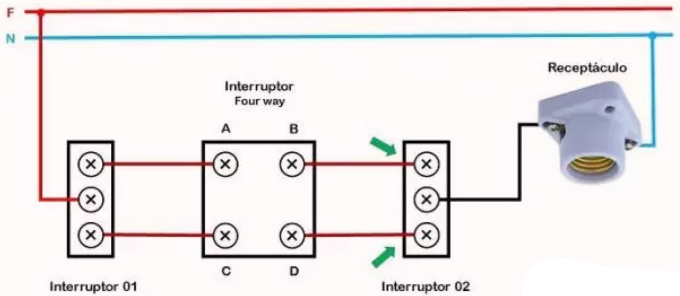
\includegraphics[width=0.8\linewidth]{Figuras/Ch08/fig25}
\end{frame}


\begin{frame}{Interruptores - Funcionamento do \textit{four way}}
	\centering
	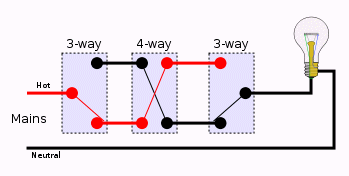
\includegraphics[width=1\linewidth]{Figuras/Ch08/fig7}
\end{frame}


\begin{frame}{Interruptores - Funcionamento do \textit{four way}}
	\centering
	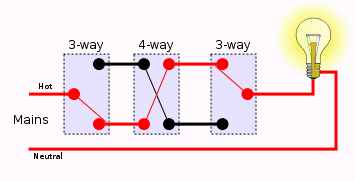
\includegraphics[width=1\linewidth]{Figuras/Ch08/fig8}
\end{frame}


\begin{frame}{Interruptores - Funcionamento do \textit{four way}}
	\centering
	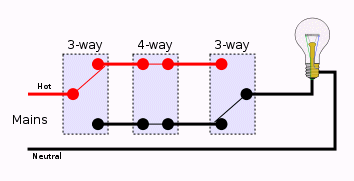
\includegraphics[width=1\linewidth]{Figuras/Ch08/fig9}
\end{frame}


\begin{frame}{Interruptores - Funcionamento do \textit{four way}}
	\centering
	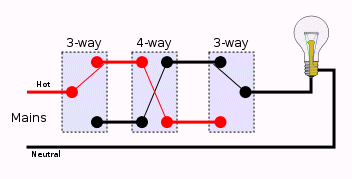
\includegraphics[width=1\linewidth]{Figuras/Ch08/fig10}
\end{frame}


\begin{frame}{Interruptores - Funcionamento do \textit{four way}}
	\centering
	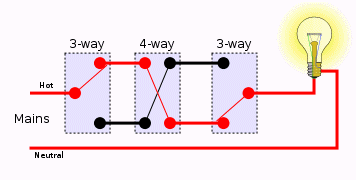
\includegraphics[width=1\linewidth]{Figuras/Ch08/fig11}
\end{frame}


\section*{Exercícios}
\frame{
	\frametitle{Exercícios}
	\begin{block}{}
		01. O que diferencia cada tipo de interruptor?

		\bigskip

		02. Quais tipos de interruptores você possui na sua casa? Faça uma lista e justifique o seu uso.
	\end{block}
}

\section*{Referências}

\frame{
	\frametitle{Referências e Exercícios Complementares}
	\begin{itemize}
		\item CREDER, Hélio; Instalações Elétricas, 14ª edição, Editora LTC, Rio de Janeiro, 2004.
		\item Manual de Instalações Elétricas - Prysmian.
	\end{itemize}
	%\centering{\alert{Página 36 - \textbf{1.6.1 até 1.6.5, 1.6.17 até 1.6.19}}} \\
	%	\centering{\alert{Lista de exercícios 01}}
}